\documentclass[11pt]{article}
\usepackage{amsmath}
\usepackage[utf8]{inputenc}
\usepackage{subcaption}%for subfigure
\usepackage{amssymb}%for tilda in math
\usepackage{float}%for forcing position of figs
\usepackage{setspace}
\usepackage{hyperref}
\usepackage{mathptmx}
\usepackage{graphicx}

\title{\large \textbf{Weekly report}}
\author{Siddharthan Rajasekaran}
\date{}
\usepackage[margin = 1in]{geometry}
 \geometry{
 a4paper,
 top = 15mm,
 }
\linespread{1}
\singlespacing
\begin{document}

\maketitle

\section{Summary}
In this report we will introduce the Metropolis Hastings sampling to compute the gradient of the likelihood and see where it fits in our algorithm



\subsection{Algorithms}

\begin{figure}[H]
  \begin{center}
    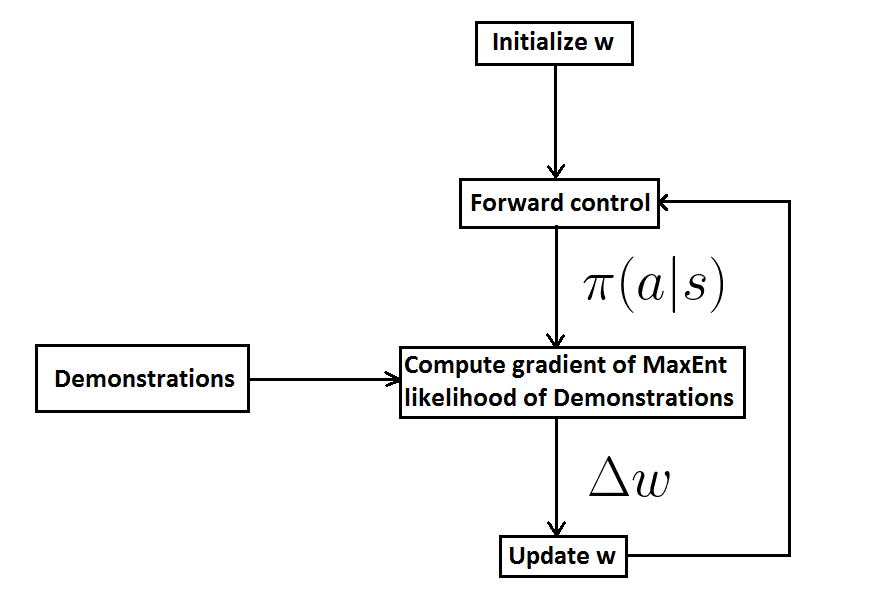
\includegraphics[width=0.7\linewidth]{images/irl.png}
    \caption{Algorithm - Maximum Entropy IRL. The Forward Control block requires a soft version of the value iteration, which is expensive to compute}
    \label{fig:cem}
  \end{center}
\end{figure}

\begin{figure}[H]
  \begin{center}
    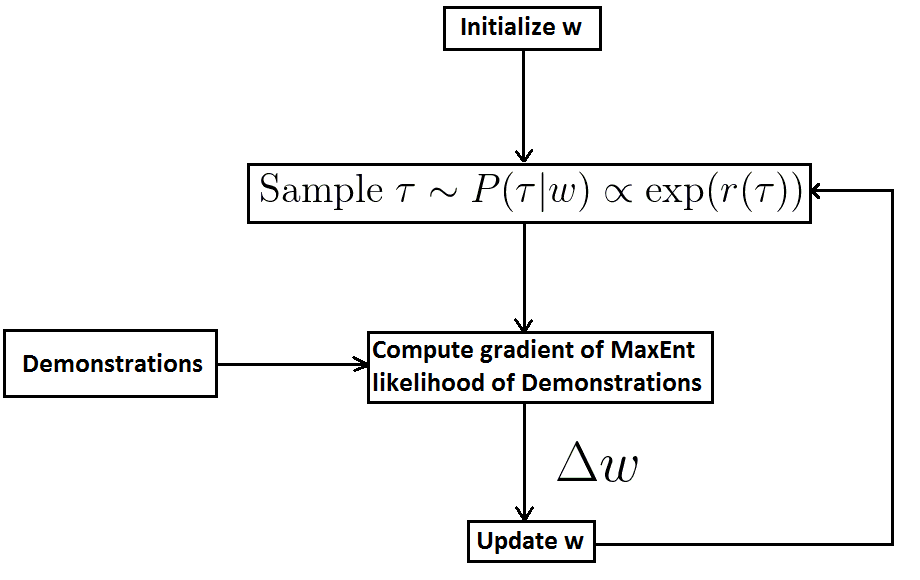
\includegraphics[width=0.7\linewidth]{images/mh.png}
    \caption{Algorithm - Maximum Entropy IRL using Metropolis-Hastings sampling. The forward control has been replaced with samples from a probability distribution proportional to exponentiated cumulative reward. Sampling from proportional distributions can be done using MH sampling}
    \label{fig:cem}
  \end{center}
\end{figure}
 

\end{document}

